
\subsection{FORTRAN I}

In 1956, they released the reference manual \citetitlecite{backus_fortran_ref_manual_1956} with a FORTRAN
that looked very similar to the original, with a few deletions and minor changes.
The ill-fated \texttt{RELABEL} formula was removed and the \texttt{DO} statement was simplified.
Instead of taking potentially three formulas (the first, last, and continuation formulas),
one now only specified the final formula of the loop, or the \gls{backedge}.

In the following loop, \texttt{I} begins at 1 and increments by 1 until it reaches 5, and for
each iteration, \texttt{N(I)} is accessed, multiplied with \texttt{I} and stored in \texttt{A(I)}:

\begin{lstlisting}[language=Fortran,frame=single]
10    DO 20 I=1,5
20    A(I) = I*N(I)
30
\end{lstlisting}

IF-statements were still quite unweildy; they took three formulas, the first if the
condition yielded a negative value, the second if it was zero, and the third if it was positive:

\begin{lstlisting}[language=Fortran,frame=single]
10    IF(A(I)) 20,30,40
20    ! ... Jump to here if A(I) < 0
30    ! ... Jump to here if A(I) = 0
40    ! ... Jump to here if A(I) > 0
\end{lstlisting}

To be fair to John Backus, he is quite self-deprecating when recalling these details about the
language design process.

\begin{quotation}
	Since our entire attitude about language design had always been a
	very casual one, the changes we felt to be desirable during the course
	of writing the compiler were made equally casually\dots

	In our naive unawareness of language design problems--of course,
	we knew nothing of many issues that were later thought to be important,
	e.g., block structure, conditional expressions, and type declarations.
\end{quotation}

At this time, Backus, Herrick, Ziller, and their team at IBM were shopping around
their compiler and programming language to potential customers of the IBM 704.
Their primary purpose was to collect aspects of the system that their customers found
confusing or objectionable, or aspects they felt were missing.
In late 1954 and early 1955, they gave talks to these customers and recieved next to
no helpful feedback.
It seemed that too frequently, customers had been systems with lots of promise, only to
finally recieve an unweildy or peculiar system with restrictions that were not mentioned
during the sales process.

The first significant payoff from these talks came in January 1955 when they visited the
United Aircraft Corporation. Roy Nutt was leased out by his boss Walter Ramshaw
to IBM to work on the input/output
libraries for FORTRAN, and he would visit New York several times a week to collaborate with
the team until 1957.
Charles Adams from MIT allowed Sheldon Best to join the team,
and Sidney Fernback from Livermore Radiation Laboratory joined as well.

Backus remarks that while his team could have been better salespeople and that
Laning and Zierler's compiler was more influential and compelling at the time, the early FORTRAN efforts
likely influenced at least the development of Hopper's Math-Matic compiler at
Sperry Rand.
If they did not convince users of the utility of their new compiler and programming language,
they at least picked up new contributors that would go on to make large contributions.

\subsection{Their First Compiler}

In early 1955 when development on their compiler began, it was only referred to as their \textit{translator}.
Herrick wrote lots of test programs to feel out the language, and the team had an ad-hoc understanding of the
sort of code they expected to get from various source programs, though their language lacked a
rigorous specification.
The team broke into smaller teams of one to three people, each responsible for a section of the compiler.
Each group agreed on the input and output formats to be used on the boundaries of their component and what came before and after.

\begin{figure}[h]
	\centering
	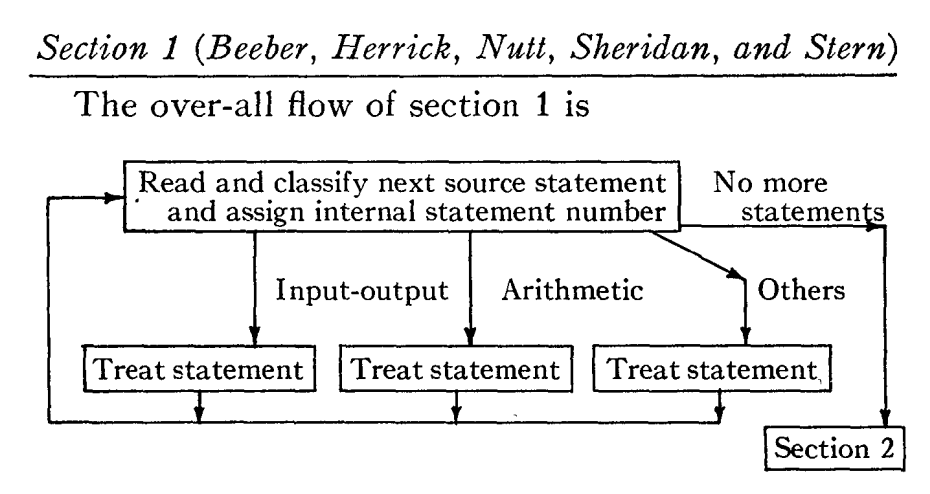
\includegraphics[width=0.8\textwidth]{resource/dawn/backus-fortran-sec-1.png}
	\caption{Section 1 of the Original FORTRAN compiler\cite{backus_etal_fortran_automatic_coding_system_1957}}
	\label{fig:backus_fortran_compiler}
\end{figure}

Their \textit{translator} was a single-pass compiler.
The first section (see Figure \ref{fig:backus_fortran_compiler}) of the compiler
consumed the entire program, produced machine code for what it could,
and left the rest of the information about the source program in lookup tables
for the other sections of the compiler.
We would likely call this the front-end of the compiler as it composed
parsing and a bit of semantic analysis.

In section 2, some parts of the user's program (particularly I/O statements)
would be transformed into DO-statements, which would then still need to be compiled.
This section also performed some optimization steps, including \gls{licm} and
register allocation.
The optimizations in section 2 were primarily invented by Robert Nelson and Irving Ziller.
These optimizations originally included register allocation \textit{for the entire program},
until Backus proposed that the earlier phases of the compiler should assume the
target machine (at this point only the IBM 704) has unlimited index registers,
and later phases of the compiler would finish the job of register allocation.

This proposal neccesitated sections 4 and 5, and section 3 to translate the
output of the first two sections into the format section 4 expected.
Lois Mitchell Haibt joined the group to design and program section 4,
which was responsible for some significant analyses.
Section 2 would be responsible for constructing and analyzing the \gls{cfg}
of the user's program, breaking the program into \gls{basicblock}s,
and \textit{performing a Monte-Carlo simulation} of the user's program
based on DO-statements and optimization hints in the form of FREQUENCY statements
to track how often each basic block was used, and to collect utilization
statistics on the program's index registers.

Wow! That must have been a massive undertaking.
Aside from inventing new compiler optimization techniques, this is the first
instance I can find of \gls{pgo}.
They quickly ran into tradeoffs between compile-time spent in analyses and optimizations
and the actual differences in performance these analyses brought to the user's
program.
In once instance, a sub-component of the register allocation analysis took ten minutes
of the twenty total minutes in compile time,
even though the program used no index registers--thus half the compile time
went towards analyses that made no difference in the final program
\cite{backus_heising_fortran_1964}.

Section 5 was then responsible for leveraging the analyses from section 4
to perform register allocation for the 704's three index registers.
This section was designed and implemented by Sheldon Best from MIT,
who was on loan as a temporary IBM employee.
Best's methods would become the basis for register allocation research for many years to come.

It was not obvious to the team until later in 1955 that a section in
between 2 and 4 would be needed; Richard Goldberg joined in November of 1955,
and he designed and implemented this section,
and took over section 5 from Best after he returned to MIT.

Section 6 was naturally designed by Nutt, as he wrote the I/O runtime libraries
for the original compiler, and section 6 assembled, linked, and loaded the final program.
For such an I/O-heavy portion of the compiler, he was the natural choice.
Thanks to the efficient I/O features Nutt added to the language, this section
was many times faster than competing assemblers and linkers.

From mid 1956 to early 1957, the focus was on bringing the compiler to market.
They would rent out a hotel near the headquarters to sleep during the day
so they could debug their new compiler all night long while it sat unused by other
teams.
The team started surprising themselves with the transformations their compiler
was capable of; the optimization gurus Nelson and Ziller would always be able to figure
out how the compiler determined the transformation was correct and beneficial, but
it was still a surprise to see all the pieces come together.

In 1957 they published a small addendum to the Programmer's Reference Manual,
documenting \textit{functions statements}, which have persisted through to modern Fortran.
They allow users to define functions in a single statement, like so:

\begin{lstlisting}
FIRSTF(X) = A*X+B
SECONDF(X, B) = A*X+B
THIRDF(D) = FIRSTF(E)/ D
FOURTHF(F,G) = SECONDF(F, THIRDF(G))
\end{lstlisting}

There were numerous language features specific to the 704 as well,
such as the SENSE LIGHT statement, which toggled specific sensor lights:

\begin{quotation}
	\begin{tabular}{|c|c|}
		\hline
		GENERAL FORM                                 & EXAMPLES      \\
		\hline
		"SENSE LIGHT i" where i is 0, 1, 2, 3, or 4. & SENSE LIGHT 3 \\
		\hline
	\end{tabular}
\end{quotation}

The PUNCH statement was also present in the handbook, which allowed users to
directly use the card-punching attachment on the 704.

Among the optimization efforts, Nelson and Ziller optimized array indexing expressions and
wrote loop analysis passes.
Backus specifies that they could "could move computations from the object
program to the compiler" which appears to be the first instance of
\gls{constant-folding} in a compiler.

In the spring of 1957, they published \citetitle{backus_etal_fortran_automatic_coding_system_1957}
and they distributed it to every IBM 704 customer.
After lots of debugging in the field and difficulties punching out copies
of the compiler, it was not long before most of the installations were using it.
By fall of 1958, more than half of the machine code produced at the roughly 70 installations
with an IBM 703 or 704 were being produced by their FORTRAN compiler.

\subsection{Optimizing FORTRAN I}

Driven by the fear of the sceptics' fears coming true and delivering a FORTRAN compiler
that produced programs significantly slower than their hand-coded equivalents,
they tried to evaluate which parts of a program would be most subject to inefficiencies.
One of the first considerations was the calculation of \textit{addressing expressions}
\cite{backus_heising_fortran_1964}
(which continues to be a challenging optimization problem).
This will be explained further below.

When a program iterates over the elements of a matrix $A_{m, n}$ with $m$ rows and $n$ columns in a loop,
the element of $A_{i, j}$ is accessed in column-major order with the following calculation:

\[
	A_{i, j} = \text{base-address}(A) + ((i - lbound(A, 1)) + m \times (j - lbound(A, 2))) \times s
\]

where $s$ is the number of bytes in an element of $A$, and $lbound$ gives the lower bound of the array
for a given dimension.
In many cases, the lower bound of all dimensions is $1$, which gives a more straightforward calculation:

\[
	A_{i, j} = \text{base-address}(A) + ((i - 1) + n \times (j - 1)) \times s
\]

And even more simply, the offset of an index from the base address of a matrix
with all-one lower bounds measured in units of the size of an element is simply:

\[
	A_{i, j} = (i - 1) + n \times (j - 1)
\]

If the loop accesses the elements of $A$ such that each element resides immediately next to the previous
element in the innermost loop, then the compiler can re-use the address calculation from the previous
iteration of the innermost loop.

More concretely, here we see the elements of our matrix $A$:
\[
	A =
	\begin{bmatrix}
		a_{1,1} & a_{1,2} & \cdots & a_{1,N} \\
		a_{2,1} & a_{2,2} & \cdots & a_{2,N} \\
		\vdots  & \vdots  & \ddots & \vdots  \\
		a_{M,1} & a_{M,2} & \cdots & a_{M,N}
	\end{bmatrix}
\]

Thus the elements are laid out in memory as a contiguous block of memory:

\[
	\big(
	a_{1,1},\; a_{2,1},\; \dots,\; a_{M,1},\;
	a_{1,2},\; a_{2,2},\; \dots,\; a_{M,2},\;
	\ldots,\;
	a_{1,N},\; \dots,\; a_{M,N}
	\big)
\]

So, a FORTRAN program accessing elements of $A$ linearly as they
are stored in memory (also known as \gls{stride1})
\href{https://godbolt.org/z/T6M4dvMP4}{would look like this:}

\begin{lstlisting}[language=Fortran,frame=single]
      real A(3,3)
      integer i,j
c     Innermost loop is the fastest-moving index
      do 10 j = 1, 3
         do 10 i = 1, 3
            A(i,j) = real(i)/real(j)
            print *, i, j
   10 continue
      end

c     Program prints:
c     1           1
c     2           1
c     3           1
c     1           2
c     2           2
c     3           2
c     1           3
c     2           3
c     3           3
\end{lstlisting}

Now, the FORTRAN team's concern was that their compiler would not be able to recognize
that a program like the one above was accessing memory in a way consistent with the
way arrays are stored in memory, and would miss the fact that in calculating
the address of an array element $A_{i,j}$ for $i > 1$, parts of the address calculation
for index $A_{i-1, j}$ could be re-used and $A_{i-1, j}$ and $A_{i, j}$ reside
next to each other in memory.

Because programmers writing machine code would naturally do this and FORTRAN
programs would spend much of their time in loops iterating over matrices,
it was critical that their compiler be able to recognize this idiom.
After scoping out the problem, they found the space of possible address calculation
expressions to be very large indeed.

For example, in the loops above, it is obvious that the matrix $A$ is accessed
with \gls{stride1} because the innermost loop iterates over the columns of the
matrix, and the \gls{inducvar} $i$ is incremented by one via the DO loop,
and is not modified in the loop body.
Consider the following program, where it is not \textit{quite} so clear:

\begin{lstlisting}[language=fortran,frame=single]
      real A(3,3)
      integer i,j
c     Innermost loop is the fastest-moving index
      do 10 j = 0, 2
         do 10 i = 1, 3
            i = i + 1
            A(i,j) = real(i)/real(j)
            print *, i, j
   10 continue
      end
\end{lstlisting}

Does this loop access $A$ with \gls{stride1}?
Yes, it does, but I hope the potential problems are becoming clear.
What if $i$ is not simply a constant offset of the innermost dimension of $A$?
What if the first index of $A$ is the result of a function call which takes $i$
as a parameter and performs some calculation based on it?
This sort of analysis would go on to be a rich subset of compiler optimization research,
and the answers are not always straightforward.
Their work on FORTRAN would become the basis for loop analyses attempting to prove
that address expressions are linear functions of \gls{inducvar}s,
permitting impactful compiler optimizations.

To match or exceed the efficiency of hand-coded loops, the group settled on a few
language restrictions that would need to be adhered to
\cite{backus_heising_fortran_1964}:

\begin{itemize}
	\item DO-loop \gls{inducvar}s must be incremented by a positive, constant integer.
	\item Array subscripts must be linear (or \textit{affine}) functions of \gls{inducvar}s.
	\item The number of subscripts must not exceed three.
	\item Control should not jump into a loop body from elsewhere in the program.
\end{itemize}

Outside of these restrictions, other were imposed for the performance of the \textit{compiler}
and not necessarily for the user's program. For example, identifiers could not
exceed six characters.
